\chapter{PLACC - Project Leader Attribution Companion and Consultant}

%\textit{Note: This chapter follows the Requirements Analysis Document Template in \cite{bruegge2004object}. \textbf{Important:} Make sure that the whole chapter is independent of the chosen technology and development platform. The idea is that you illustrate concepts, taxonomies and relationships of the application domain independent of the solution domain! Cite \cite{bruegge2004object} several times in this chapter.}

As seen in the previous chapters, the research conducted in the topic of Attribution Theory in Software Engineering Team Management has produced valuable insights and results.  Such knowledge could be beneficial to a larger audience,  and therefore, motivated the creation of a tool, intended to be used by future project leaders or anyone interested in the topics of this thesis. We decided to name this tool PLACC, which is an abbreviation for \textit{Project Leader Attribution Companion and Consultant}. Although the solution we provide is a prototype based on the findings in this thesis, this prototype can be further extended to include more empirical data.  An overview with the motivation is included in \ref{Overview}, whereas the requirements elicited for the product can be found in \ref{Requirements}. The models representing PLACC will conclude this chapter in \ref{SystemModels}.
We assume that the majority of the users will be project leaders, therefore, we will be utilizing them often as representatives of the users throughout this chapter as we further describe PLACC. 

\section{Overview} \label{Overview}

As the name itself suggests,  with PLACC we aimed at defining and developing a tool which would offer interested parties a variety of overarching information.  PLACC would now only present project leaders with inappropriate behaviours and their corresponding attribution biases, but also provide data and best practices on dealing with them. We envisioned PLACC to consult project leaders especially when a situation seems disturbing to them or if they are confused on how to assess a certain behaviour. 
Furthermore, considering that many project leaders were willing to share their tips and tricks for the virtual setting, we decided to add a second "C", standing for Companion. This addition serves exactly the purpose of guiding especially young PLs in their endeavours, with an emphasis at the activities at the beginning of projects.

The main motivation for the development of such a tool, were the project leaders themselves (current and future). The virtual setting introduces challenges unthinkable before (as described in \ref{VirtualLeadership}),  which have been subject to research for two decades now and continue to yield new insights. Our goal is to address the challenges concerning wrongful and unnecessary perceptions of project leaders, by making the knowledge we have gathered more accessible. Throughout the interviews, the project leaders shared an interest in a centralized pool of data, which we hope to have been materialized, at least to some extent, through PLACC.

\section{Requirements Elicitation} \label{Requirements}

In this section we will elaborate on the application domain and define requirements in more detail. We will start with user stories, which describe the system from the point of view of the user and are concerned with adequately representing their needs. The user of PLACC is primarily the project leader, but an extended version of PLACC also considers the developer and the researcher as users. Next, we will advance with requirement elicitation, by showcasing the functional and non-functional requirements the system under development should fulfil. The source of these requirements are the project leaders, which would express their desires during the interviews.  Next, we will discuss more advanced topics of requirements elicitation such as scenarios and use case model. 

\subsection{User Stories}

Considering that the literature and projects surrounding the attribution bias in the management software engineering projects is limited, we considered it necessary to formulate user stories that capture the desired outcome and the reason for wanting that specific outcome.  In Extreme Programming, user stories are used in the early phases of planning and they represent requirements which are elicited and written with the client.  Stories are high-level use cases that encompass a set of coherent features.  The structure of the following user stories follows the one described in the agile software development literature, such as in \cite{Cohn2004}.  

As briefly described in the introduction of this section, the origin of the user stories are the project leaders themselves. During the interviews, numerous project leaders would express their interest in the topic, suggesting functionalities and preferences. These requirements are compiled together and represented through the following user stories:

\begin{itemize}
\item As a project leader, I want to be introduced to behaviours that can potentially bias me, so that I can better prepare for what awaits me.

\item As a project leader, I want to see how other project leaders have perceived the person exhibiting an inappropriate situation (to me) so that I can compare my experience to theirs.

\item As a project leader, I want to be provided with suggestions on how to deal with a certain situation, so that I can apply this knowledge in real projects.

\item As a project leader, I want to be acquainted with variations of main types of behaviours, so that I can be aware of a broader spectrum of behaviours.

\item As a project leader, I want to be able to differentiate between data retrieved from different sources or methods, so that the source of the information is more transparent to me. 

\item As a project leader, I want to read a "manual" of what to keep in mind especially in the first weeks of leading a project, so that I can minimize unpleasant experiences in the future.

\item As a project leader, I want to learn about the real reasons behind a behaviour, so that I can adjust my reaction accordingly. 

\end{itemize}

User stories also represent functionality that the system must offer to the users.  They are organized into stacks of related functionality and the list above is already prioritized to fit the needs of the users. More on the way \textit{how} these can be realized, will be described in the next subsection. 

\subsection{Functional Requirements} \label{FunctionalRequirements}

%\textit{Note: List and describe all functional requirements of your system. Also mention requirements that you were not able to realize. The short title should be in the form ``verb objective''}

Functional requirements describe the interactions between the system and its environment independent of its implementation \cite{bruegge2004object}.  We will be basing the functional requirements on the user stories presented above and the descriptions also follow the examples in \cite{bruegge2004object} .

\begin{itemize}
\item [FR1] \textbf{Browse behaviours}: The user should be able to browse through a catalogue of behaviours.  The title of the behaviour must be easily distinguishable and the items of the catalogue can be chosen for further reading.
\item [FR2] \textbf{Examine behaviour details}: The user should be provided with various details associated with a behaviour.  The most important details include a list of attribution as well as suggestions on how to deal with the behaviour. It must be noted that a behaviour might be exhibited in different variations, which are in themselves also behaviours. PLACC behaviour details should also be backed up with the source of the information presented.
%\item [FR3] \textbf{Explore personas}: Personas can be attached to various behaviours, and the user should have the opportunity to learn more about them. 
\item [FR3] \textbf{Learn from former PL experience}: Young PLs should have a designated place with suggestions and recommendations about virtual project management.  PLACC contains and prepares a compilation of such experiences to be accessible by everyone.
\item [FR4] \textbf{Follow tutorial}: The users should be provided with a designated space in which they learn more about the purpose of PLACC and how to navigate through the app. The tutorial should be presented to the users the first time they use the app, and be accessible anytime in the app too.
\end{itemize}

We were able to identify one more functionality, which unfortunately could not become part of the implementation of PLACC. Regardless, this functionality would contribute to the richness,  validity and extensibility of the application, and is described in the following functional requirement:

\begin{itemize}
\item [FR5] \textbf{Share own experience}: The users should be integral part of the PLACC database of behaviours and attributions. This is achieved by allowing the users to provide their own experiences. PLACC takes these experiences into consideration when putting the app data at the users' disposal.
\end{itemize}

\subsection{Nonfunctional Requirements}

%\textit{Note: List and describe all nonfunctional requirements of your system. Also mention requirements that you were not able to realize. Categorize them using the FURPS+ model described in \cite{bruegge2004object} without the category \textbf{functionality} that was already covered with the functional requirements.}

In this section we will elaborate on the nonfunctional requirements of PLACC. Before diving into them, we want to denote that PLACC is not meant for commercial use, and is not currently supposed to distributed in a production environment. 

\begin{itemize}
\item [NFR1] \textbf{Usability}: Since the topics of PLACC are very domain specific, the mode of use should be explained in a manual-like text.
\item [NFR2] \textbf{Usability}: The presentation should unfold in a friendly, human-centered design.
\item [NFR3] \textbf{Usability}: There is no need for authentication when reading the PLACC data.
\item [NFR4] \textbf{Maintenance,  Extensibility}: The system should be built in such a way,  that can be easily extensible in the future with more behaviours and their accompanying attributes.
\item [NFR5] \textbf{Performance}: The system should immediately register user input and present in the PLACC UI.
\end{itemize}

Furthermore, we have identified the following pseudo-requirements:

\begin{itemize}
\item [PR1] \textbf{Implementation}: In order to practically visualize the results and stay within the language constraints of the iPraktikum, this application will be developed in \textit{Swift},  relying on the library of SwiftUI as interface builder.
\item [PR2] \textbf{Operation}: The source data must be stored in a format that can be easily read and written by humans.  This data must be accessible and manageable from the researchers of PLACC, in order to guarantee data integrity.
\end{itemize}


\section{System Models} \label{SystemModels}

%\textit{Note: This section includes important system models for the requirements analysis.}

According to \cite{bruegge2004object}, system models describe the scenarios, use cases, object model, and dynamic models of the system. This section contains the complete functional specification,  starting from the scenarios and concluding with mock-ups illustrating the user interface of the system and navigational paths representing the sequence of screens.  In this chapter we will refrain from the dynamic models, as there is no direct or complex interaction between the participants of the system.

\subsection{Scenarios}

%\textit{Note: If you do not distinguish between visionary and demo scenarios, you can remove the two subsubsections below and list all scenarios here.}

After defining the requirements of the system and identifying the actors,  it is beneficial to describe features as in a narration, in order to better understand the steps and interactions with the system.  A scenario fulfils such purposes and it is a concrete, informal description from the viewpoint of a single actor. There will be two types of scenarios presented in this section: \textit{visionary} and \textit{demo} scenarios.

PLACC is primarily intended to demonstrate the findings of the case study,  but the numerous behaviours,  attributions and personas are indicators that these topics can be extended even more.  Therefore,  we describe in visionary scenarios an idealized and futuristic version of the system.  The demo scenario will present what realistically could be accomplished within the scope of this thesis.

Regarding the actors, the most prominent one is the project leader, who not only makes use of the data of PLACC, but also contributes to its value.  Other actors include the developer and the researcher.

In the scenarios with project leader as an actor, the motivation and entry points are the same.  A project leader identifies a behaviour which they consider to be subjectively inappropriate, and turn to PLACC to learn more about the behaviour and how it can be addressed.

\subsubsection{Visionary Scenarios}

%\textit{Note: Describe 1-2 visionary scenario here, i.e. a scenario that would perfectly solve your problem, even if it might not be realizable. use our scenario description template in form of a table.}

The visionary PLACC system does not only provide information to the interested user but also includes their input as part of the calculated and presented data.  The following scenarios explain two ways this can be realized,  with two distinct actors. 

\begin{longtable}[ht]{ p{0.20\textwidth}  p{0.75\textwidth} }
\caption{\texttt{inappropriateBehaviorDetected} Visionary Scenario}
\label{tab:firstVisionaryScenario}\\
\hline
\textit{Scenario name} & \underline{\texttt{inappropriateBehaviorDetected}} \\ [1.2ex]
    \hline
   \textit{Actors} & \underline{\texttt{Anna: Project Leader}}  \\ [1.2ex]
   \hline
   \textit{Flow of events } &  1. Anna detects an unusual behaviour in her virtual team and turns to PLACC. She is asked to select from a list of behaviours or to enter her own identified behaviour. She finds the behaviour of \textit{wearing an inappropriate attire} in the list. \\
   & 2. Anna needs to enter two more fields. She need to answer how she feels about the behaviour and to reason about the motivation and the causes. She can then submit this data and proceed to reading about the behaviour. \\
   & 3. Anna is faced with a personalized set of information to her. She firstly reads statistics about her own attribution and then proceeds to read about the perceptions other people might have created.  Additionally, the system provides what other PLs think the cause of the behaviour is. \\
   & 4. Anna is also presented with an estimation of the \textit{actual} reason behind the behaviour, which does not include other PLs perceptions. \\
   & 5. Anna has now learned that the reason for this behaviour is probably a comfortability of the person exhibiting this behaviour. This behaviour is not intended to disrespect anyone, which was the way she initially felt. Anna knows 30\% of PLs also do not appreciate this behaviour and learns from them that this issue can be addressed in the meeting opener. \\
   \hline
\label{tab:multicol}
\end{longtable}

The second visionary scenario achieves similar results as the previous one,  but from the subject's point of view. The subject in this case is the member whose behaviour is being perceived by the project leader a certain way. In the context of the iPraktikum, the subject is a developer. 

\begin{longtable}[ht]{ p{0.20\textwidth}  p{0.75\textwidth} }
\caption{\texttt{argueBehaviourReason} Visionary Scenario}
\label{tab:secondVisionaryScenario}\\
\hline
\textit{Title} & \underline{\texttt{argueBehaviourReason}} \\ [1.2ex]
    \hline
   \textit{Actors} & \underline{\texttt{Tom: Developer}} \\ [1.2ex]
   \hline
   \textit{Flow of events } &  1. Tom is a developer who listens about PLACC in one of his lectures and wants to contribute to it.  He is asked to select from a list a behaviour that he has consciously exhibited before.  Tom selects the behaviour of \textit{communicating with another person in the room} from the list. \\
   & 2.  Tom is then required to answer the question: \textit{What was the reason behind this behaviour?} He replies saying that no one would notice him talking to another person,  and that he did not think it would be considered abnormal.  He then submits this data.\\
   & 3. He is then being presented with statistics regarding the above selected behaviour from the PLs points of view.  Tom reads through them,  and realizes that his behaviour might be more inappropriate than what he thinks.  75\% of PLs think this behaviour is unprofessional, while 60\% think it is disrespectful towards the participants of the team.\\
   \hline
\label{tab:multicol}
\end{longtable}

The actors in these visionary scenarios are actively collaborating to the improvement of PLACC.  The second scenario especially does not only take in consideration the perceptions of the PLs,  but takes into account input from the other members of the team as well, hopefully providing bidirectional benefits.  

The intention behind this scenario,  is that quite often the perceptions we create as humans are not correspondent to reality,  and gaining insights directly from the source, can reject the (false) hypothesis the human brain creates.  From the developer's point of view,  a behaviour might be exhibited as they do not realize the impact it has in the perception PLs or other team members create.  

This knowledge would help all stakeholders prevent an escalation of events or deeper misunderstandings. Awareness is described in \cite{Trainer2018} as an important contributor in building trust and improving team collaboration. We believe that a version of PLACC supporting the above-described scenarios would achieve a higher awareness between the participants.  Furthermore, the system described in these scenarios is intended to be self-sufficient and unreliable on manual interpretation of input data. 

\subsubsection{Demo Scenarios}

%\textit{Note: Describe 1-2 demo scenario here, i.e. a scenario that you can implement and demonstrate until the end of your thesis. use our scenario description template in form of a table.}

The following demo scenarios provide a more feasible expectation from PLACC and are part of the version we were able to deliver.  The first scenario describes the process of getting acquainted with the attributes of a behaviour which disturbs the project leader.

\begin{longtable}[ht]{ p{0.20\textwidth}  p{0.75\textwidth} }
\caption{\texttt{disturbingBehaviourInTeam} Demo Scenario}
\label{tab:disturbingBehaviourInTeam}\\
\hline
\textit{Title} & \underline{\texttt{disturbingBehaviourInTeam}}\\ [1.2ex]
    \hline
   \textit{Actors} & \underline{\texttt{Anna: Project Leader}} \\ [1.2ex]
   \hline
   \textit{Flow of events} &  1. Anna is very surprised to see how quiet everyone is in the meetings and turns to PLACC to learn more about this situations. She is presented with a list of behaviours she can choose from. She finds the behaviour of \textit{Lack of audible participation} in the list which fits her situation and clicks on it to learn more. \\
   & 2. Anna has the opportunity to choose between different variations of the behaviour that provide a bit more context. She clicks on one of the variations which reads "Stays muted almost all the time". \\
   & 3. Anna can read about the attributions others have formed, and see where her opinion stands in comparison to others.  She realizes that just as her, 85\% of her colleagues consider this behaviour to be unprofessional. \\
   & 4. Anna reads about suggestions on how to deal with this specific behaviour and makes a decision. \\
   & 5. Anna is more clarified now and is relieved to see other PLs share the same opinion. She is also more confident in her next steps.  \\
   \hline
\label{tab:multicol}
\end{longtable}

The following scenario describes the situation of a project leader being faced with the responsibility of managing a virtual team.  In this scenario we assume that the app is an additional source for the management of virtual teams, which can be distributed or presented to project leaders at the beginning of projects. 

\begin{longtable}[ht]{ p{0.20\textwidth}  p{0.75\textwidth} }
\caption{\texttt{newVirtualProject} Demo Scenario}
\label{tab:newVirtualProject}\\
\hline
\textit{Title} & \underline{\texttt{newVirtualProject}} \\ [1.2ex]
    \hline
   \textit{Actors} & \underline{\texttt{Emma: Project Leader}} \\ [1.2ex]
   \hline
   \textit{Flow of events} &  1. Emma is a young project leader who is assigned the job of managing a virtual team.  Among other resources, she learns that PLACC offers an aggregation of advice from previous project leaders.  She downloads the app. \\
   & 2.  Emma is presented with a tutorial which explains the information architecture of PLACC.  Although the focus seems to be on behaviours and attributions, it is too early for her to be concerned with such issues.  Additionally, the app does offer tips and tricks for young project leaders in a designated area. \\
   & 3. Emma navigates to that area and continues to read about the typical challenges  of remote teams and how to address them.\\
   & 4. Emma is clearer now about the atmosphere of the first weeks of the project, and is determined to create a healthy social relationship within the team. \\
   \hline
\label{tab:multicol}
\end{longtable}

The fundamental difference between the visionary scenarios and the demo is the addition of features which automate the process of gathering data manually from project leaders or students. A generic solution to these differences will be presented in the Use Case Model.

\subsection{Use Case Model}

%\textit{Note: This subsection should contain a UML Use Case Diagram including roles and their use cases. You can use colors to indicate priorities. Think about splitting the diagram into multiple ones if you have more than 10 use cases.
%\textbf{Important:} Make sure to describe the most important use cases using the use case table template. Also describe the rationale of the use case model, i.e. why you modeled it like you show it in the diagram.}

After presenting the scenarios,  in this section we will be defining and describing a use case model that better determines the scope of the actor-system interaction.  Use cases generalize scenarios and clarify to the developer the tasks of the system under development.  

Additionally,  attaching use cases to initiating actors enables developers to acknowledge the roles of the different users. Often, by focusing on who initiates each use case, developers identify new actors that have been previously overlooked.  Similarly to the scenarios, a crucial activity before deriving the use cases of our system, is to identify the actors that will interact with it.  

The~\nameref{fig:UseCaseModel} in~\autoref{fig:UseCaseModel} presents the use cases distinguished in the analysis of PLACC, as well as the participating actors and the relationships between them.

In the process of identifying the actors,  we have recognized the \textbf{DataProvider} and the \textbf{ProjectLeader}. In our case, we introduce the role of the \textbf{DataProvider} as the initiator of the use case, as it is them who has previously conducted the research provides the initial data. This actor is a typical generalization, as they might be the researcher,  as in the current case, or fellow project leaders and developers who input their data into the app directly, as elaborated in the visionary scenarios. 

\begin{figure}
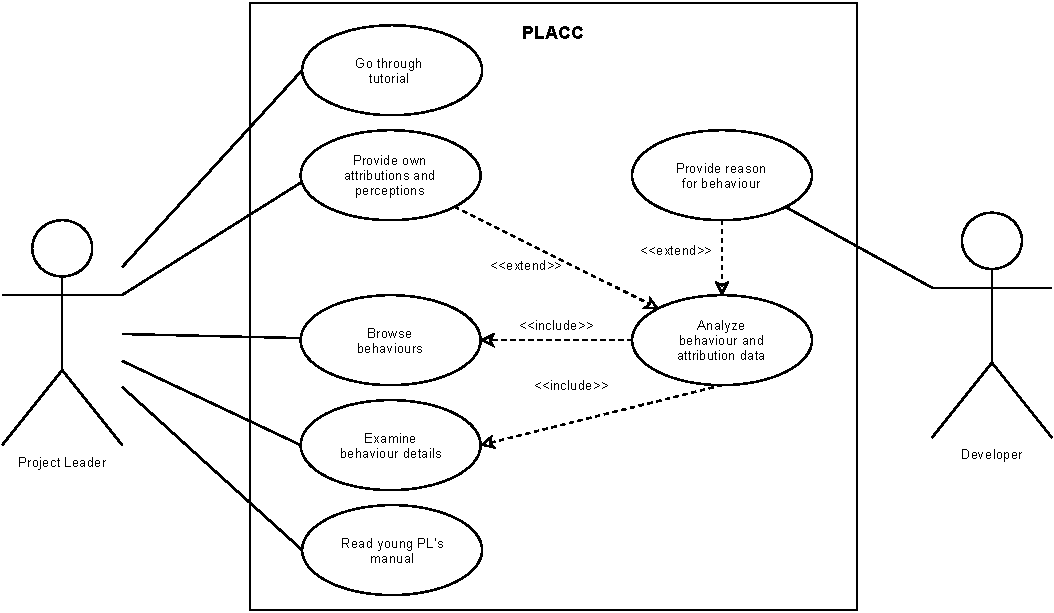
\includegraphics[width= \textwidth]{figures/UseCaseModel.pdf}
\caption{Use Case Model}
\label{fig:UseCaseModel}
\end{figure}

Logically,  PLACC cannot exist without the core behaviour data provided by e.g.  a researcher. Therefore,  starting from the top right corner of the use case model (see~\autoref{fig:UseCaseModel}), the initiatory use case would be \textbf{ProvideAttributionData}.  This data is then processed by PLACC to be readable and understandable from the end-user of the system.  The object of \textbf{AnalysisData} is concerned with exactly this issue and represents the processed set of data.  It is the system itself that supports the preparation of the data and places the data at the disposal of the user.  Therefore, the relationship between \textbf{ProvideAttributionData} and \textbf{AnalysisData} is denoted with include,  as the \textbf{AnalysisData} must be preceded by an input or injection.

From the \textbf{ProjectLeader's} perspective,  they should be able to follow a tutorial within the app, in order to understand the motivation behind PLACC and the structure of the application.  This is the first step a PL must go through, as they are not informed on the nature of the study and the different ways they can profit from PLACC.

Upon learning more about PLACC and its range of knowledge, the project leader can \textbf{BrowseBehaviours} to find a behaviour they are particularly interested in.  It can also be that the project leader is curious about PLACC, wants to explore the findings of the research.  Next,  they can choose to \textbf{ExamineBehaviourDetails}.  With this use case, the project leader can dive into the results of the research and learn about the behaviour's variations, attributions and personas.

In order for the data to be examined by the project leader, they should be previously processed and prepared for visualization. For that reason, a \textit{<<include>>} relationship exists between \textbf{BrowseBehaviours}, \textbf{ExamineBehaviourDetails} and the object of \textbf{AnalysisData}. These relationships denote that, in order for the user to browse behaviours or a single behaviour,  the input data is pre-processed following the logic provided by PLACC and prepared for visualization. The \textbf{AnalysisData} should contain behaviours, attributions and personas.

Another use case of PLACC is the opportunity to learn from the experience of previous project leaders. This activity is represented via the use case of \textbf{ReadPLManual}. The manual should elaborate on the experience as a virtual leader of software development teams and provide advice on the situation.

We will elaborate two of the use cases in the next tables. The first use case is a generalization of the two visionary scenarios, and represents a high-level solution intended to include both. 

\begin{longtable}[ht]{ p{0.20\textwidth}  p{0.75\textwidth} }
\caption{\texttt{ProvideAttributionData} Use Case}
\label{tab:UseCase}\\
\hline
\textit{Name} &  \texttt{ProvideAttributionData} \\
    \hline
   \textit{Participating actors} & Initiated by \texttt{DataProvider} \\
   \hline
   \textit{Flow of events} &  1.  The DataProvider goes into the system to input their own data. \\
   & \vspace{-1.5pc}\begin{enumerate}
   \item [2.]  The PLACC system presents a designated interface in which the DataProvider can make their contribution.  The interface supports a variety of behaviours and the attached questions in a form.  
   \end{enumerate} \\
   & 3.  The DataProvider chooses a specific behaviour and answers the questions. They also submit the answers.  \\
   & \vspace{-1.5pc}\begin{enumerate}
   \item [4.] The system stores the new data and processes the input into the AnaysisData, which will then be presented to the other users of PLACC.
   \end{enumerate} \\
   \hline
    \textit{Entry conditions} &  App is downloaded. \\
    \hline
     \textit{Exit conditions} &  The contribution made my the DataProvider is available directly to the users of PLACC. \\
      \hline
\label{tab:multicol}
\end{longtable}

The second use case we decided to present relates to the display of the core information of PLACC.  A ProjectLeader makes use of PLACC to learn more about an inappropriate behaviour, including variations, attributions and advice.  Table \ref{tab:UseCaseTwo} represents the circumstances and the flow of actions leading to the fulfilment of the ProjectLeader's goal.

\begin{longtable}[ht]{ p{0.20\textwidth}  p{0.75\textwidth} }
\caption{\texttt{ExamineBehaviourDetails} Use Case}
\label{tab:UseCaseTwo}\\
\hline
\textit{Name} & \texttt{ExamineBehaviourDetails} \\
    \hline
   \textit{Participating actors} & Initiated by \texttt{ProjectLeader} \\
   \hline
   \textit{Flow of events} &  1.  The ProjectLeader selects one of the behaviours for further examination. \\
   &  \vspace{-1.5pc}\begin{enumerate}
   \item [2.] The PLACC system opens a new view presenting initial content of an behaviour including variations. 
   \end{enumerate} \\
   & 3.  The ProjectLeader reads through the different variations of a behaviour and opens one of them. \\
   & \vspace{-1.5pc}\begin{enumerate}
   \item [4.]  The variation is expanded to accommodate other data such as personas, attributions etc. 
   \end{enumerate} \\
   & 5. The ProjectLeader goes through the details of the variation of choice. \\
   \hline
   \textit{Entry conditions} &  Sufficient AnalysisData is available. \\
    \hline
     \textit{Exit conditions} &  None \\
      \hline
\label{tab:multicol}
\end{longtable}

We decided to focus of these two use cases as they depict an indirect interaction between ProjectLeaders and DataProviders and satisfy a big part of the requirements from the system. 


\subsection{Analysis Object Model}

%\textit{Note: This subsection should contain a UML Class Diagram showing the most important objects, attributes, methods and relations of your application domain including taxonomies using specification inheritance (see \cite{bruegge2004object}). Do not insert objects, attributes or methods of the solution domain.
%\textbf{Important:} Make sure to describe the analysis object model thoroughly in the text so that readers are able to understand the diagram. Also write about the rationale how and why you modeled the concepts like this.}

~\autoref{fig:AOM} depicts the \textit{Analysis Object Model (AOM)} of the system under development. The AOM represents the main objects and the relationships that exist among them from the user's point of view.  As specified in \cite{bruegge2004object}, the AOM serves as a visual dictionary of the concepts participating in the system and its objects are to be identified in the use cases. 

As PLACC combines project leader needs and this thesis's results, the AOM also combines objects from both these sources. The paragraphs to come will describe the analysis object model following a top-down approach.

Not only the AOM,  but also the ideation of this thesis started from observing agile software development \textbf{teams} and the dynamics that emerge between its participants. The teams we observe are distributed and operate using means of remote communication and collaboration. Meetings are held on Zoom, communication takes place in platforms such as RocketChat or Discord and screensharing and remote control facilitate group collaboration especially in development tasks. The team follows the structure, guidelines and processes of Scrum \footnote{https://www.scrum.org/resources/what-is-scrum}.

\begin{figure}
	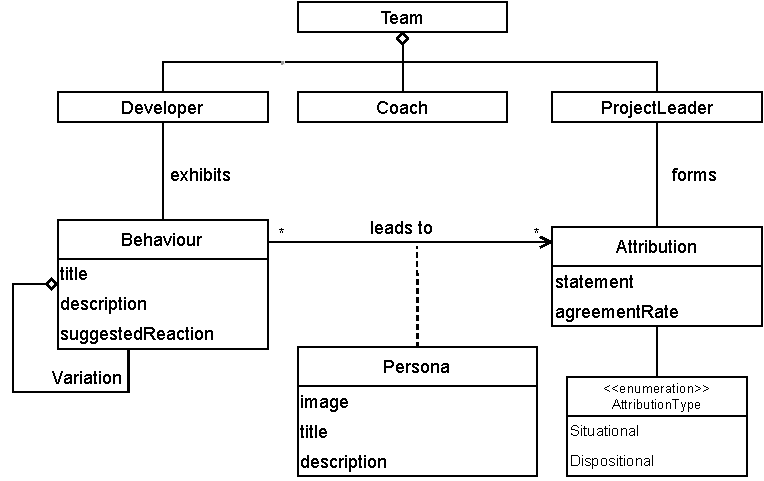
\includegraphics[]{figures/AOM2.pdf}
	\caption{Analysis Object Model}
	\label{fig:AOM}
\end{figure}

The iPraktikum teams consist of the \textbf{project leader}, \textbf{coach} and \textbf{the developers}. The project leader serves as the product owner and is responsible for communicating and reinforcing the product goals into the team. The coach represents the scrum master, and makes sure that the scrum principles are maintained. The scrum developers are responsible for providing increments until eventually building the product. In the semester in which this case study took place, there were 1-2 project leaders and coaches per team. 

Although every human being acts and expresses oneself via \textbf{behaviours}, we are specifically interested in the ones exhibited by the developers of the team. We consider the relation between the developers and the project leaders the more interesting to observe, as their competences are distinct and as the project leader has a more distant relationship to the team. This is contrasting to the position of the coach, who needs to stay closer to team.

After the interviews with the project leaders and the process of building a taxonomy of behaviours, it was identified that, although some behaviours were similar in their core, they could also vary depending on the context or circumstances. This taxonomy was constructed as an attempt to understand the domain, and we concluded that broader behaviours consist of more specific \textbf{variations}.

We judged that a behaviour consists of a title, a description and a suggested reaction towards this behaviour. Normally a behaviour is characterized by numerous other properties, but these three are the ones we consider.

Other important properties such as motivation or reason of a behaviour are not studied directly, but rather indirectly as part of the \textbf{attributions} project leaders form. Similarly to behaviours, everyone is capable of forming attributions, but the project leaders are taken into consideration as the subjects of the study. Attributions are formed as a developer exhibits a behaviour, usually new or different from what the perceiver (in our case the PL) is used to see. 

An attribution is expressed by a statement, and embodies the reasoning behind the causes of a behaviour. Considering that the survey described in \autoref{chap:Survey} also served the validation and quantification of attributions, we were able to retrieve the frequency of the agreeing responses to each attribution. Although we have retrieved other metrics in regards to an attribution, the agreement rate is the one we deemed as interesting for the users of PLACC. The agreement rate makes it possible to identify \textbf{personas} too.

Although different researchers use different conventions,  we simplify different attribution types by focusing on situational and dispositional attributions.  These are also represented in the enumeration \textbf{AttributionType}. If the \textbf{attribution type} is situational, it means that the project leaders take in consideration the situation and circumstances of the developer when forming an attribution. Dispositional attribution happens, when the disposition of the developer is considered as the cause of a behaviour. The disposition included character, personality and demeanour.

A behaviour can lead to multiple attributions, and a attribution (e.g. bad internet connection) can be used as an excuse to many behaviours. In this system we focus rather on the first association between the two objects, hence, the unidirectional arrow in the model. 

In the intersection of behaviours and attributions is where \textbf{personas} will be found. A persona is a personification of an individual which exhibits a certain set of behaviours, and is perceived a specific way by the project leaders. A persona has a title, usually a short and striking one, and a description that gives more details. An image is also associated with a persona, is order to add a visual element as well.   

\subsection{UI Mockups}

One important aspect of system analysis is also contemplating the user interface with which PLACC will be presented.  We decided to follow a lean and modern design, with few accents of colour and rich imagery. The UI aims at conveying the novelty and quirkiness of the thesis,  and tries to make it more approachable and friendly with the human elements in the graphic design.

These arguments motivated the choice of a sans serif font for the modelling of the mock-ups,  a font style which symbolizes modernity, approachability and cleanness. The accent colour of choice is purple as it is associated with wisdom, independence and magic and can evoke creativity.

Not only did this phase help with envisioning PLACC, but we were also able to identify omissions in the functional requirements. Such a case were the personas, which we intended to include in the behaviours, but did not receive a specific requirement.  Since the functional requirements were inspired by the project leaders, they had no information regarding personas, during the interviews.  Therefore,  such a gap in the requirements was to be expected.

~\autoref{tab:mockups} depicts three out of 4 tabs of the application. Since the behaviours and their details are of importance, we have dedicated more space to showcasing this view of the application. The open tab can be noticed by the coloured tab item at the bottom of the views. 

The order of the tab represents also the order of importance. The two first tabs are associated directly with the core objective and deliverables of this thesis, whereas the last two ones represent manual-like information. 

The last tab of the application is reserved as a tutorial for the new users of PLACC. We assume that the user is not acquainted with PLACC, its purpose and elements. Therefore, we take this place to elaborate on them, and to enable a more straightforward navigation through the app. The first part of the view will be dedicated to the research behind PLACC,  emphasizing its objectives.  The following sections will explain each tab of the application in detail, starting from the personas and finishing with the Young Project Leader's Manual.  


\pagebreak
\begin{longtable}[ht]{ p{0.05\textwidth} p{0.45\textwidth}  p{0.45\textwidth} }
\caption{UI Mock-ups}
\label{tab:mockups}\\
    \hline
    \textbf{Name} & \textbf{Mock-up}& \textbf{Description} \\
    \hline
 \multirow{1}{*}[-2.5cm]{\rotatebox{90}{\textbf{Browse behaviours}}} & 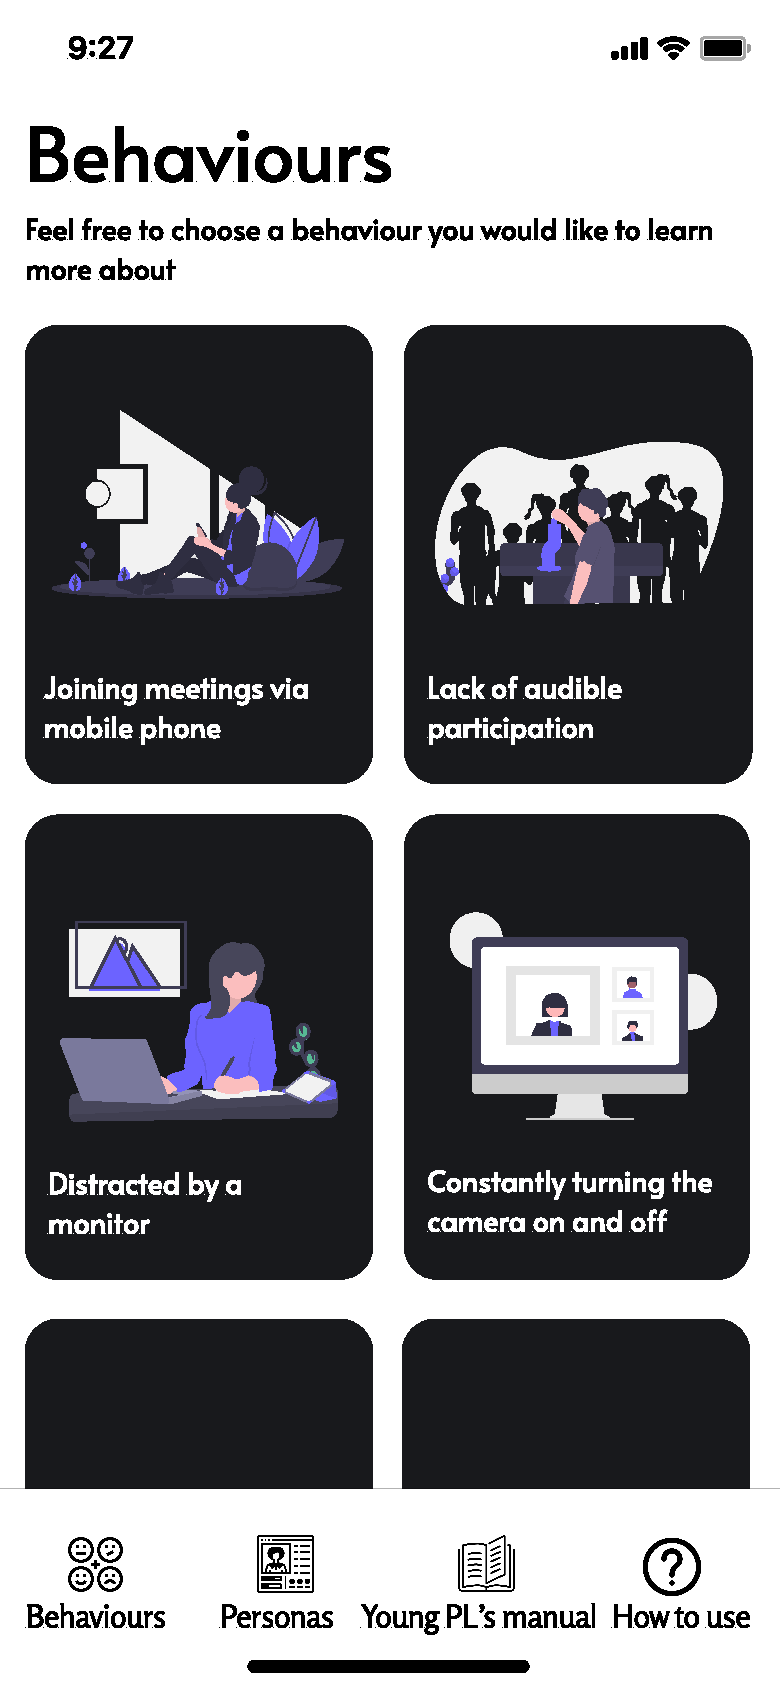
\includegraphics[valign=t,  width=1.55in]{figures/Behaviours.pdf} & The first tab of the application presents a grid of cards, each constituting and redirecting to a behaviour.  Each card contains a representative image and the title of the behaviour. \\
   \hline
  \multirow{1}{*}[-2.2cm]{\rotatebox{90}{\textbf{Explore behaviour details}}}  & 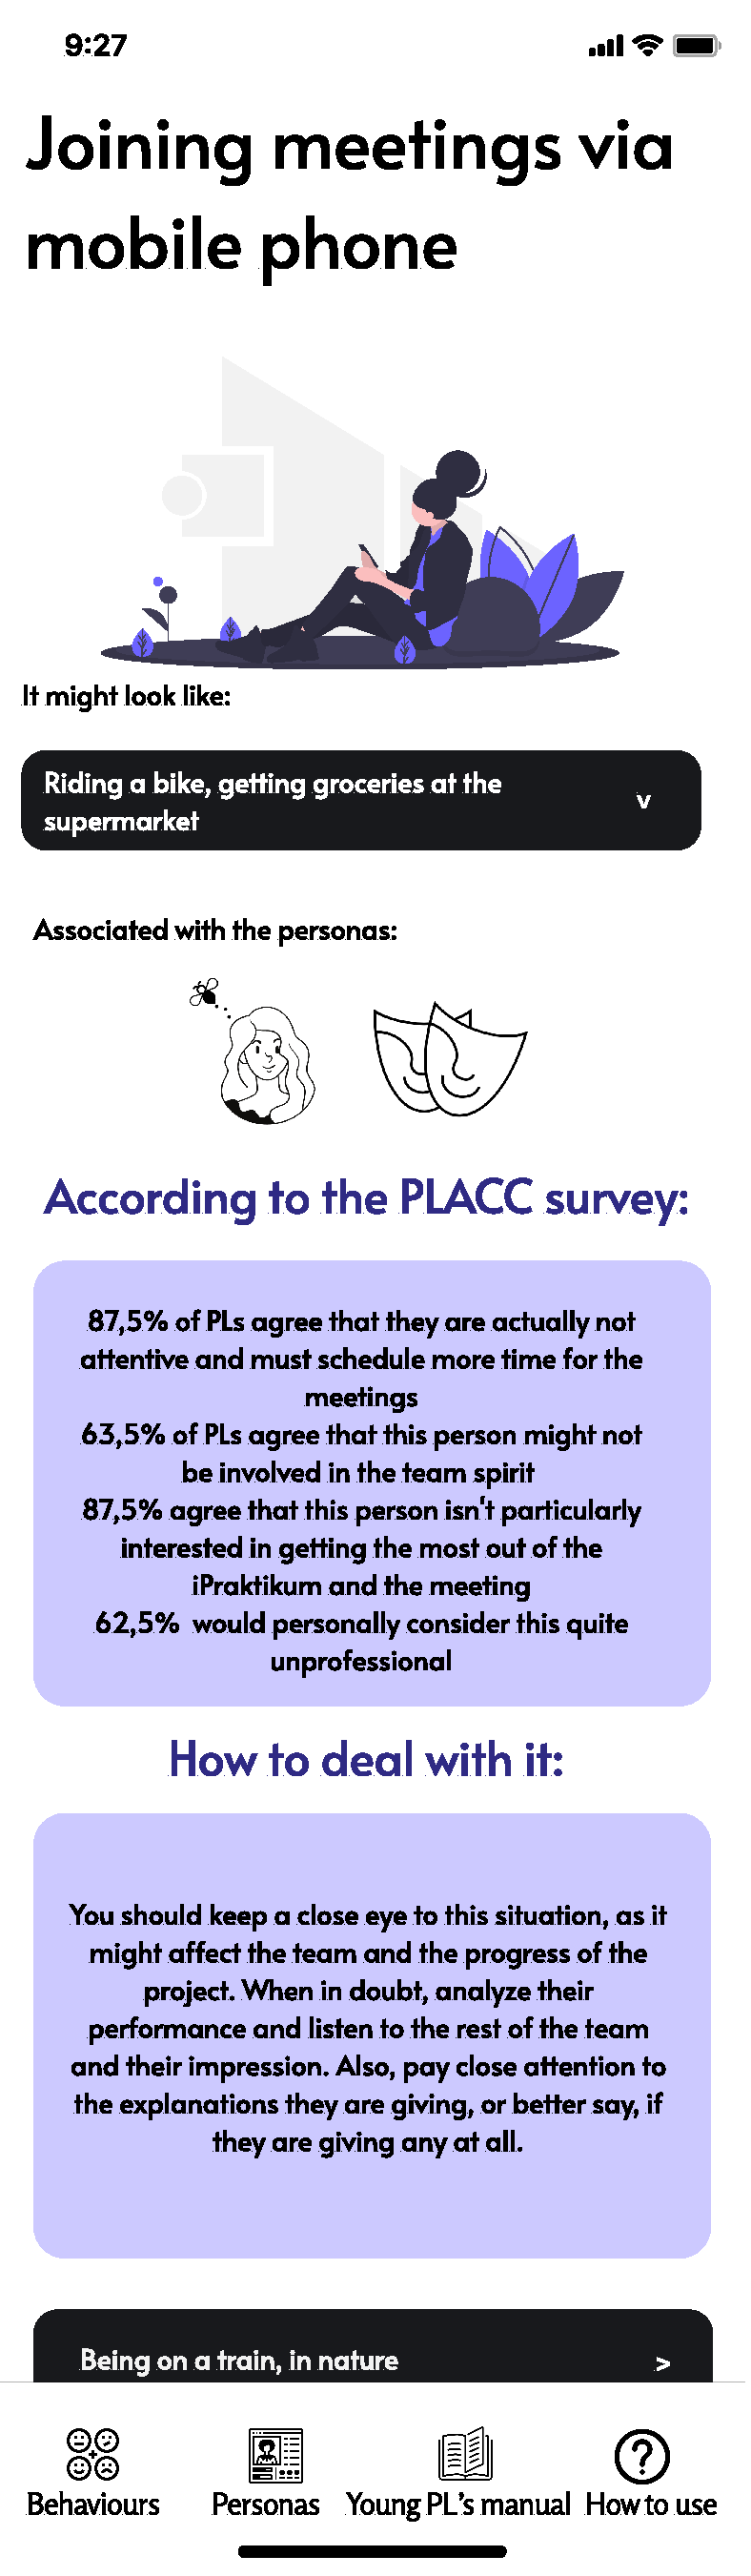
\includegraphics[valign=t, width=1.55in]{figures/ASpecificBehaviour.pdf}   &  Upon choosing one of the behaviours,  the user will be presented with a detailed behaviour view.  Every behaviour will be distinguished in further variations,  containing personas,  attributions and suggested solutions or reactions towards that behaviour.  In this first screenshot of the view we can see a variation of the behaviour in the black button.  We see the open version of the variation which includes personas and the beginning of the attributions made part of the survey. \\
    \hline
    \multirow{1}{*}[-1cm]{\rotatebox{90}{\textbf{Explore behaviour details (continuation)}}}  & 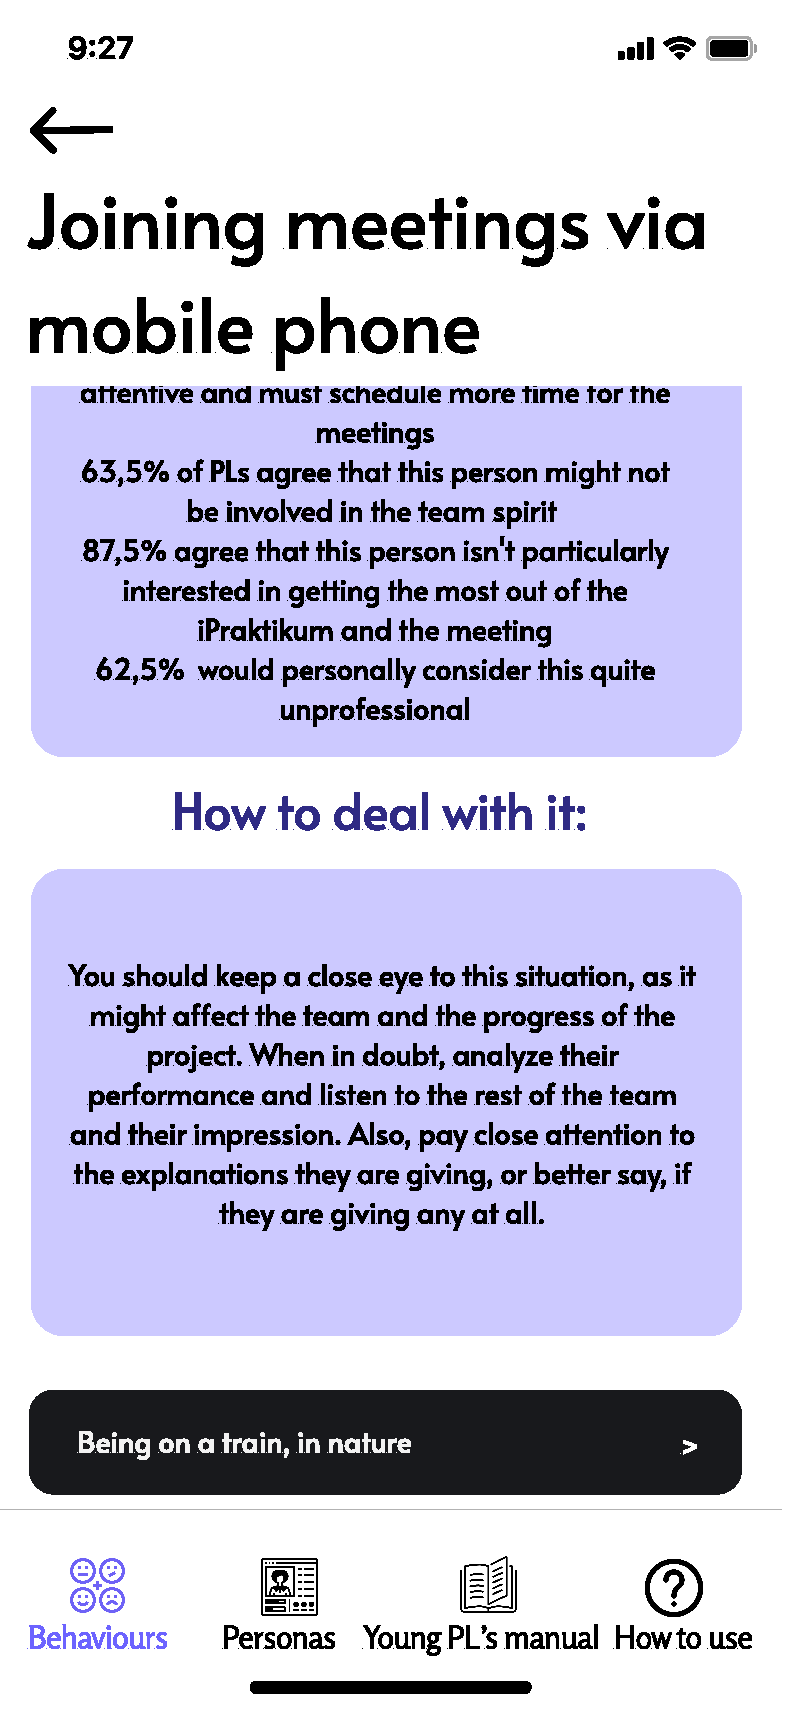
\includegraphics[valign=t, width=1.6in]{figures/ASpecificBehaviourPart2.pdf}   & The user will not only we able to learn and assess attributions, but also be presented with suggestions on how to deal with this behaviour. This is shown in the second block of the variation data.  Afterwards, the user can choose to open the second variation (at the bottom of the screen) or navigate back to the behaviour card grid (arrow at the top-left corner) \\
    \hline
    \multirow{1}{*}[-3.5cm]{\rotatebox{90}{\textbf{Personas}}} & 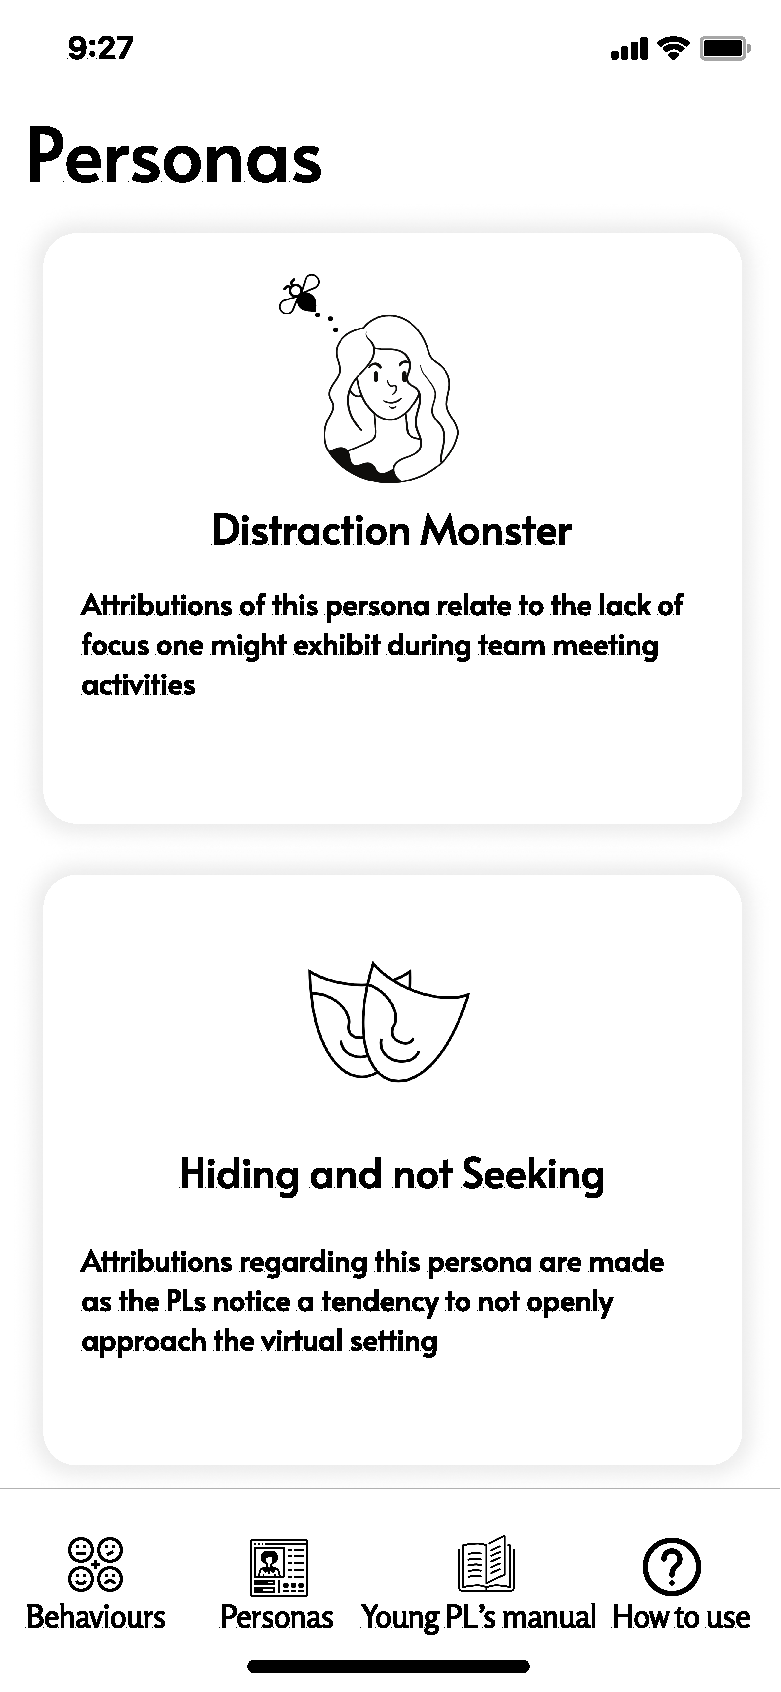
\includegraphics[valign=t, width=1.6in]{figures/Personas.pdf} &  As personas will be part of a behaviour's description,  the second tab of the application will be dedicated to the explanation of personas. 	These are also represented via cards, and contain an image (which can be found in the behaviour details), the title and a description of the persona.\\
   \hline
    \multirow{1}{*}[-2.5cm]{\rotatebox{90}{\textbf{Young PL's Manual}}} & 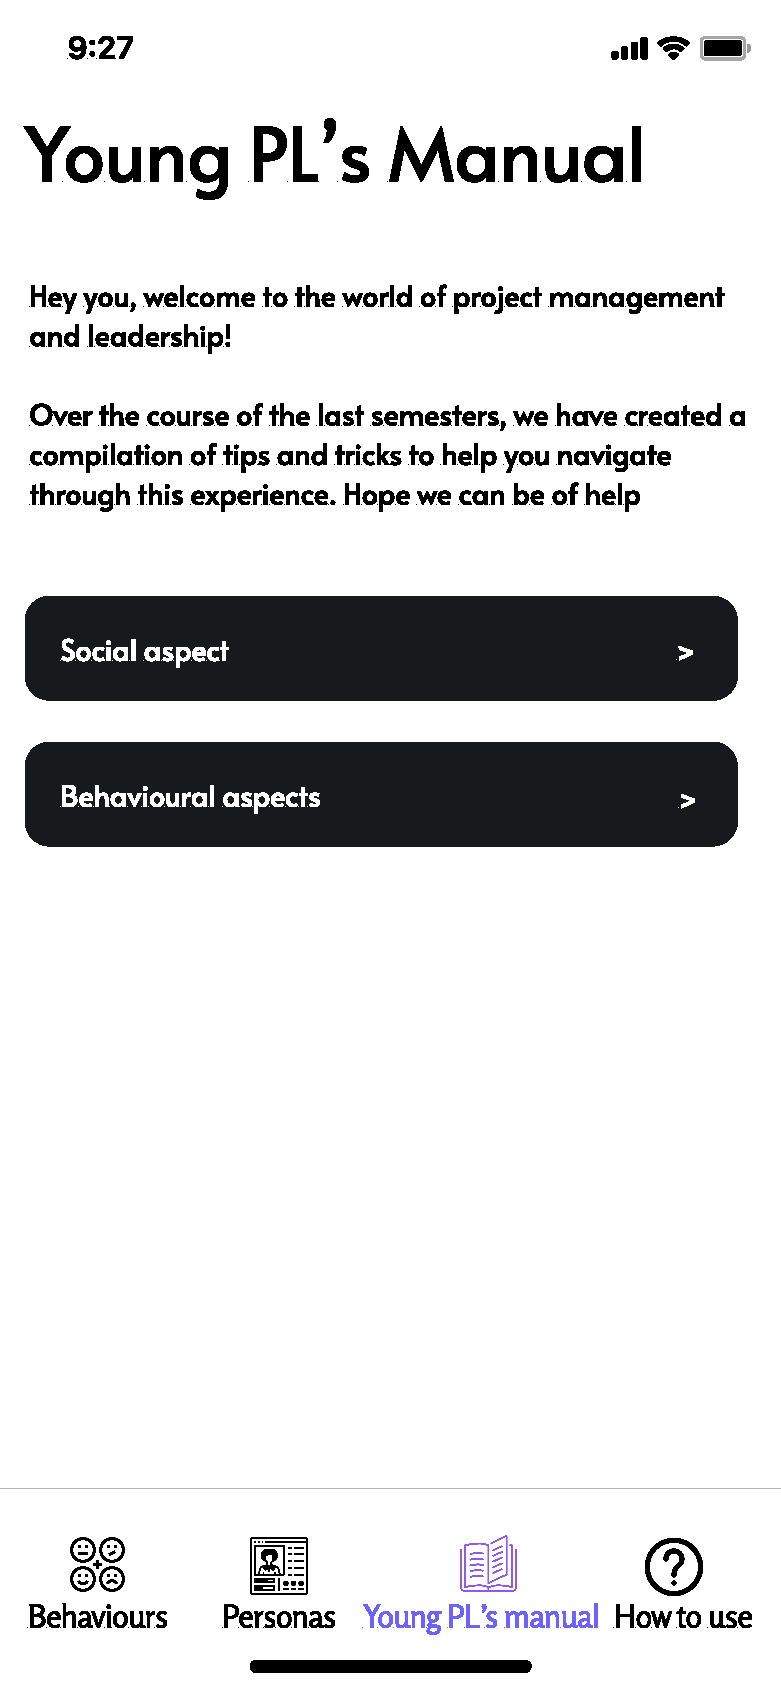
\includegraphics[valign=t, width=1.6in]{figures/HowTo.pdf}  &  Considering the knowledge we have gathered in this thesis,  want to offer young PLs a space in which they can read about previous leadership experience and tips on how to deal with specific situations.  The information is categorized in sections, using the same button design and behaviour of the variation. \\
   \hline
\label{tab:multicol}
\end{longtable}
